\documentclass{beamer}

\usepackage{metalogo}
\usepackage{hologo}

\usepackage{graphicx}
    \graphicspath{{./img/}}

\usepackage{polyglossia}
	\setmainlanguage{english}

\usepackage{fontspec}
	\defaultfontfeatures{Mapping=tex-text}
	\setmainfont{FreeSans}
	\setsansfont{FreeSans}
	\setmonofont{FreeMono}
	\setromanfont[Renderer=ICU]{Charis SIL}

\usepackage{ctable,multicol,multirow,array,color,etoolbox}
\usepackage{listings}
	\lstset{frame = single,
	   numbers = left,
	   breaklines = true,
	   breakindent = 0pt,
	   basicstyle=\ttfamily}

%%%%%%%%%%%%%%%
%%%% STYLE %%%%
%%%%%%%%%%%%%%%

\usetheme{Szeged}
\usecolortheme{beaver}

\setbeamertemplate{caption}[numbered]
\setbeamertemplate{section in toc}[sections numbered]
\setbeamertemplate{subsection in toc}[subsections numbered]
\setbeamertemplate{footline}
{%
  \begin{beamercolorbox}[colsep=1.5pt]{upper separation line foot}
  \end{beamercolorbox}
  \hbox{%
    \begin{beamercolorbox}[wd=0.333333\paperwidth, ht=2.5ex, dp=1.125ex, center]{title in head/foot}%
      \usebeamerfont{author in head/foot}\insertshortauthor
    \end{beamercolorbox}%
    \begin{beamercolorbox}[wd=0.333333\paperwidth, ht=2.5ex, dp=1.125ex, center]{title in head/foot}%
      \usebeamerfont{title in head/foot}\insertshorttitle
    \end{beamercolorbox}%
    \begin{beamercolorbox}[wd=0.333333\paperwidth, ht=2.5ex, dp=1.125ex, center]{title in head/foot}%
      \usebeamerfont{title in head/foot}\insertframenumber/\inserttotalframenumber\hspace*{2ex}
    \end{beamercolorbox}}
  \begin{beamercolorbox}[colsep=1.5pt]{lower separation line foot}
  \end{beamercolorbox}
}


\title[Introduction to \hologo{BibTeX}]{Introduction to \hologo{BibTeX}: reference management in \XeLaTeX}
\author{Stefano Coretta}
\date{February 11, 2016}

%%%%%%%%%%%%%%%%
%%% DOCUMENT %%%
%%%%%%%%%%%%%%%%


\begin{document}

%%%%%%%%%%%%%%%%%%%%%%%%%%%%%%%%%%%

\begin{frame}
	\maketitle
\end{frame}

%%%%%%%%%%%%%%%%%%%%%%%%%%%%%%%%%%%

\section{Introduction}

\begin{frame}
    \frametitle{What is \hologo{BibTeX}?}

\begin{itemize}
    \item \hologo{BibTeX} is a \textbf{reference management system} based on \TeX{}
    \item it is also a \textbf{format} with which you write a bibliographical database
    \item so it is \textit{both} a software (\texttt{bibtex} engine) and a format (\hologo{BibTeX})
    \item to use it, you need
    \begin{itemize}
    \item a \texttt{.bib} file, which contains your bibliographical database
    \item a \texttt{.bst} file, which specifies the reference style
    \end{itemize}
\end{itemize}

\end{frame}

%%%%%%%%%%%%%%%%%%%%%%%%%%%%%%%%%%%

\begin{frame}[fragile]
    \frametitle{How does it work?}

\begin{itemize}
    \item you first insert your entries in the \texttt{.bib} file
    \item each entry has a unique cite key (like \texttt{asimov1951} for Asimov's \textit{Foundation})
    \item in your \texttt{.tex} file, you cite the references in your text using the \verb+\cite+ command and the cite key of the entry you are citing
    \item you compile using the \texttt{bibtex} engine
    \item \hologo{BibTeX} takes care of inserting the citation and the reference list with the appropriate formatting, as specified in the \texttt{.bst} file
\end{itemize}

\end{frame}

%%%%%%%%%%%%%%%%%%%%%%%%%%%%%%%%%%%

\begin{frame}
    \frametitle{\hologo{BibTeX} front-ends}

Creating your bibliographical database (\texttt{.bib}) can be facilitated using a front-end:

\begin{itemize}
    \item BibDesk (Mac only)
    \item JabRef
    \item Mendeley Desktop
    \item EndNote
    \item Zotero
\end{itemize}

\end{frame}

%%%%%%%%%%%%%%%%%%%%%%%%%%%%%%%%%%%

\section{How to}

%%%%%%%%%%%%%%%%%%%%%%%%%%%%%%%%%%%

\begin{frame}
    \frametitle{BibDesk}

\begin{figure}
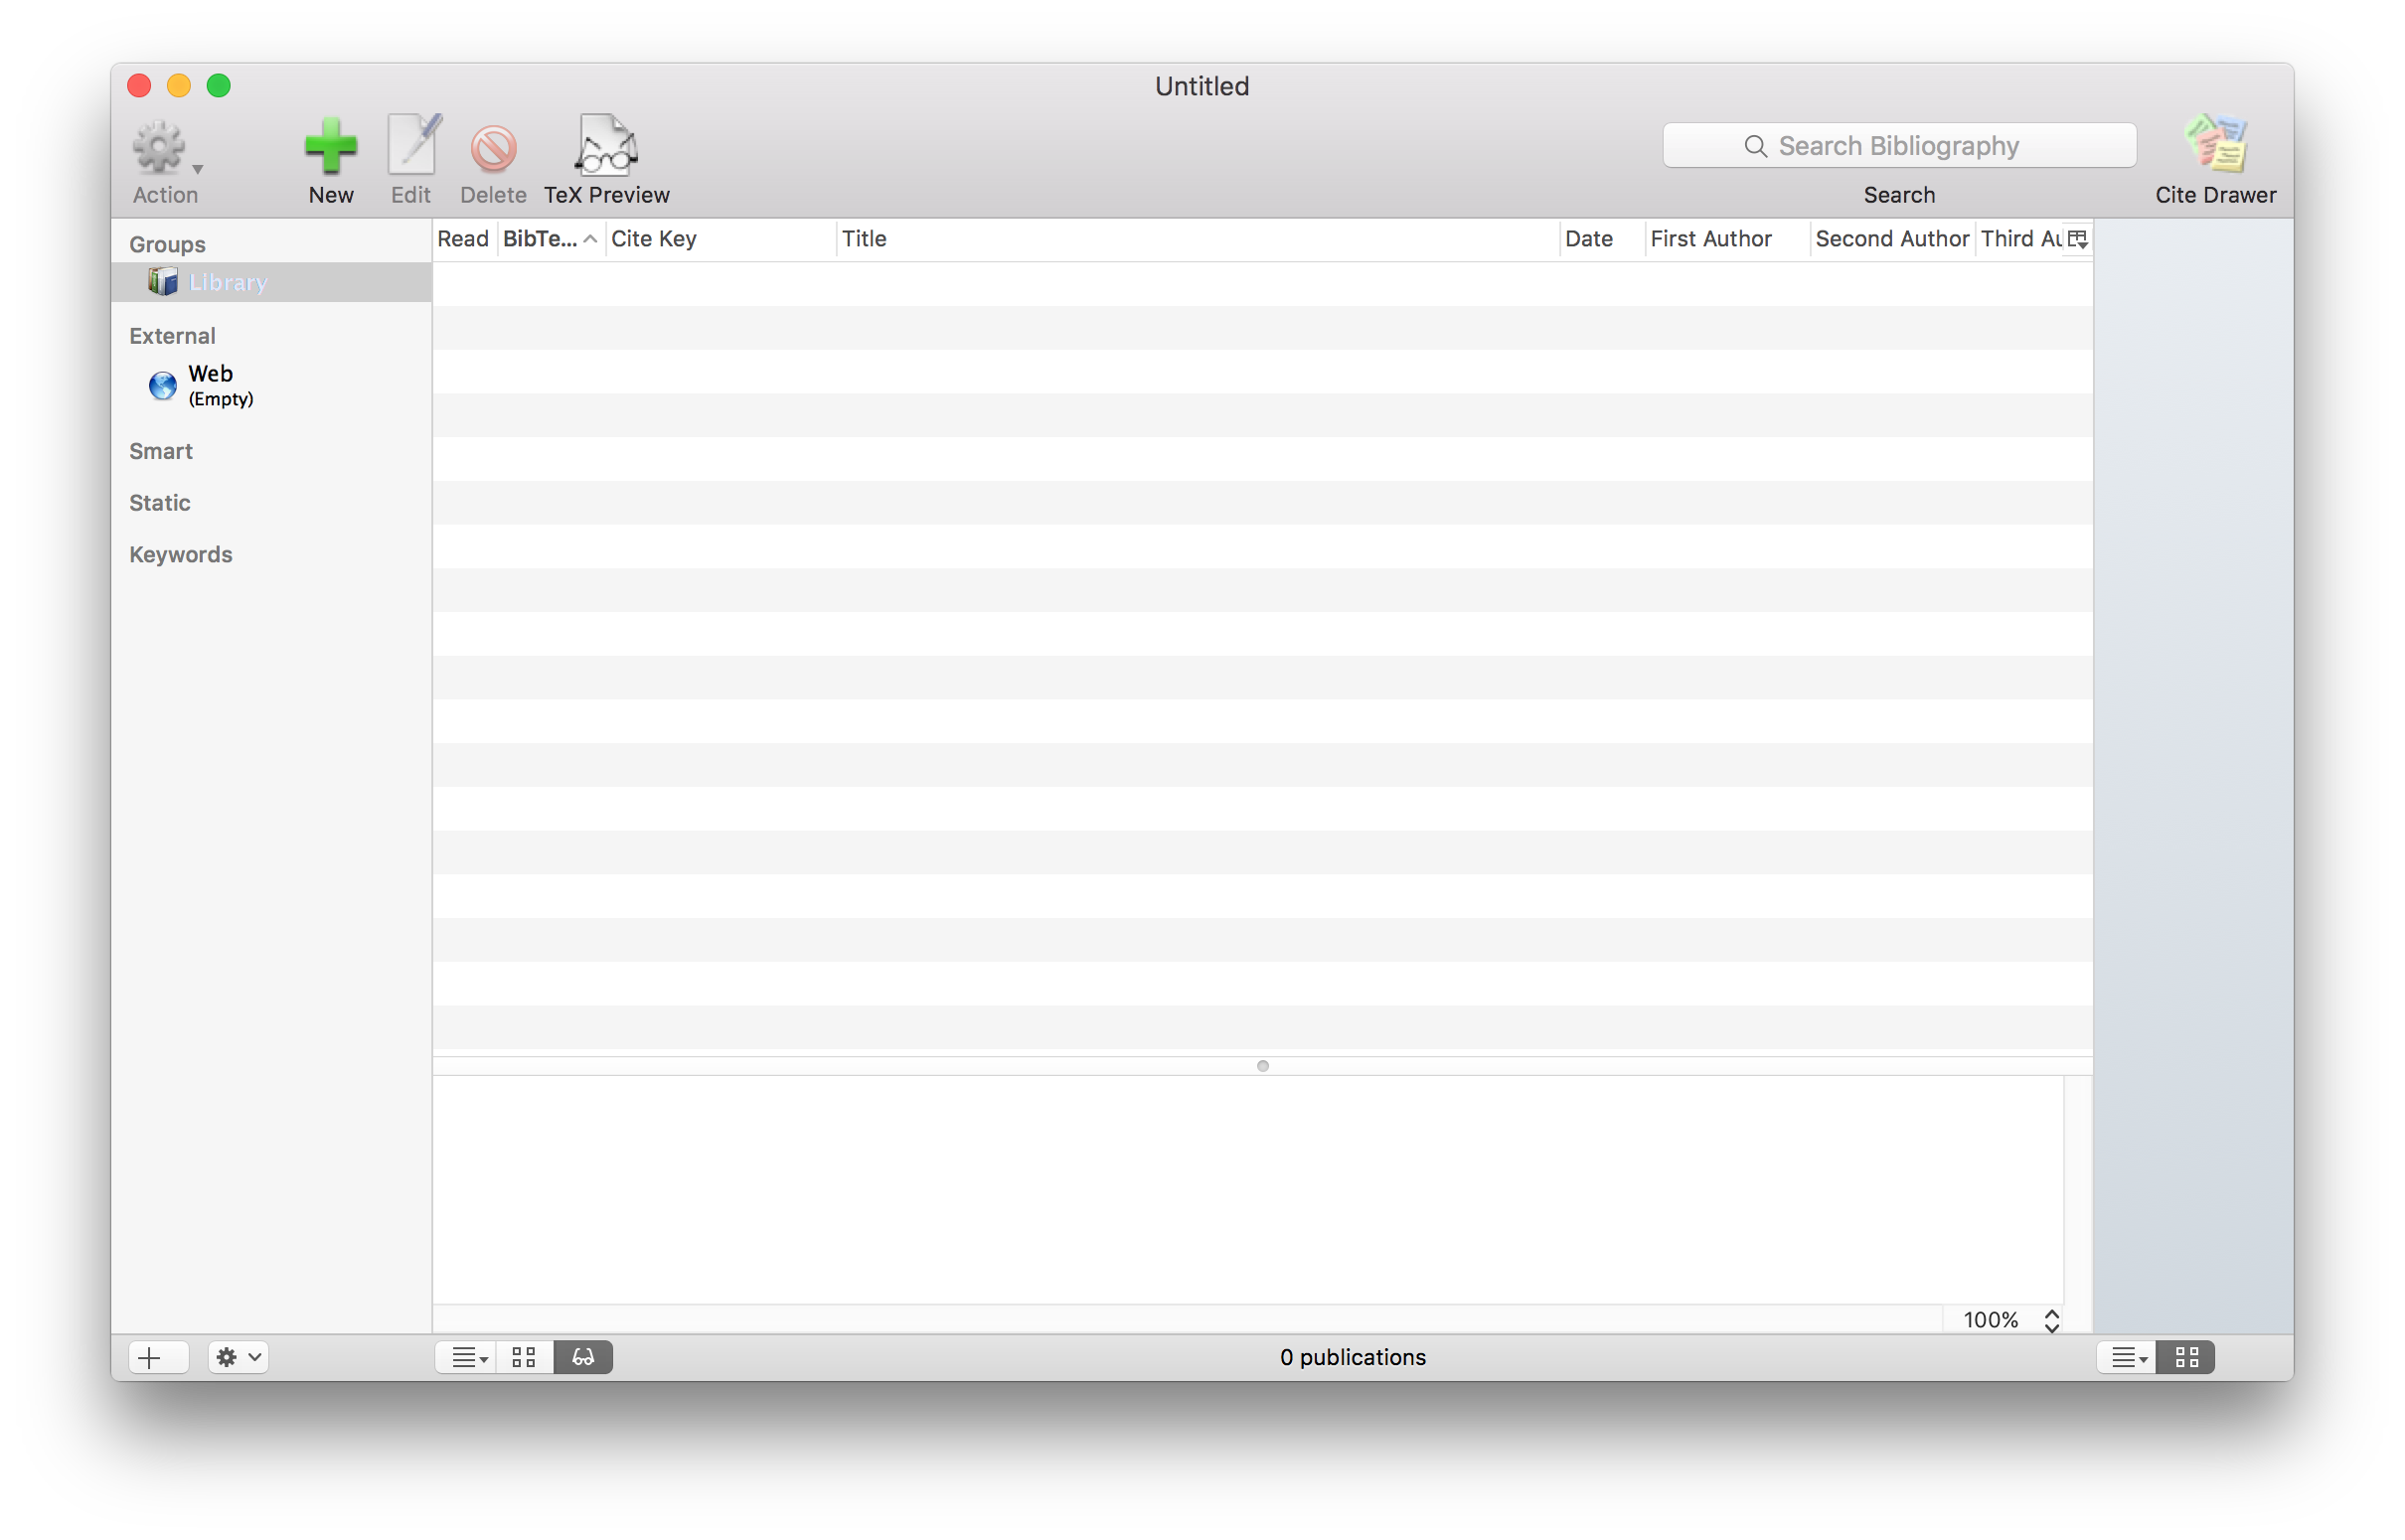
\includegraphics[width=\textwidth]{bibdesk}
\caption{BibDesk: a front-end for \hologo{BibTeX}.}
\label{f:bibdesk}
\end{figure}

\end{frame}


%%%%%%%%%%%%%%%%%%%%%%%%%%%%%%%%%%%

\begin{frame}
    \frametitle{BibDesk}

\begin{figure}
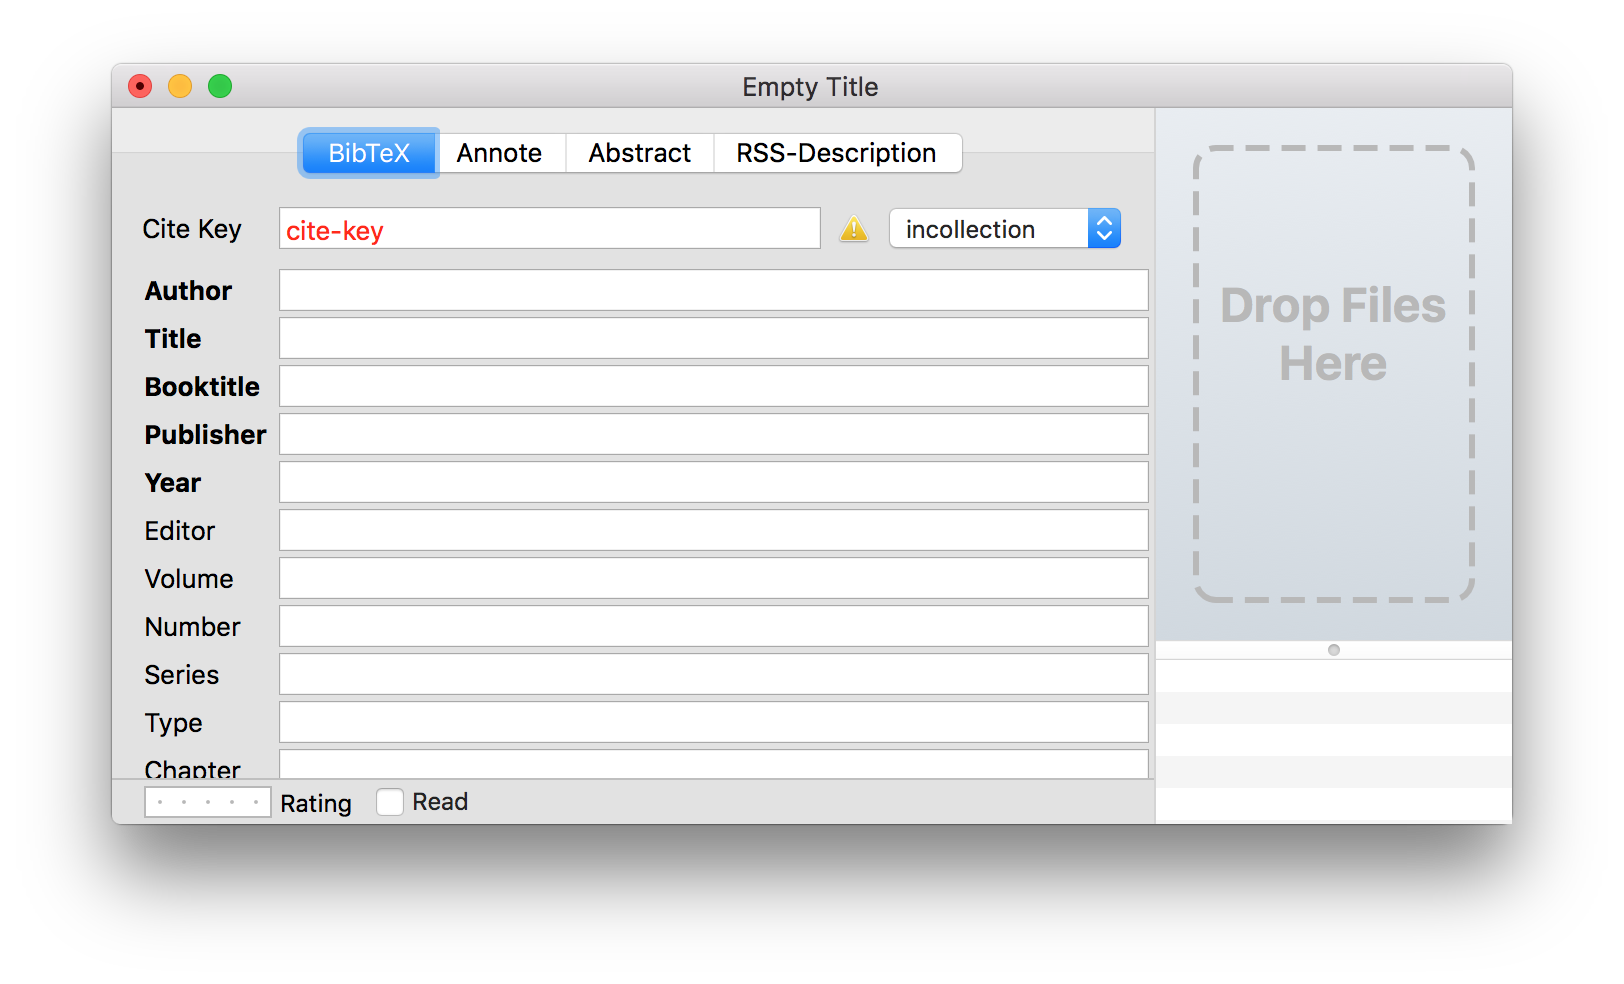
\includegraphics[width=\textwidth]{new-entry}
\label{f:bibdesk}
\end{figure}

\end{frame}

%%%%%%%%%%%%%%%%%%%%%%%%%%%%%%%%%%%

\begin{frame}
    \frametitle{BibDesk}

\begin{figure}
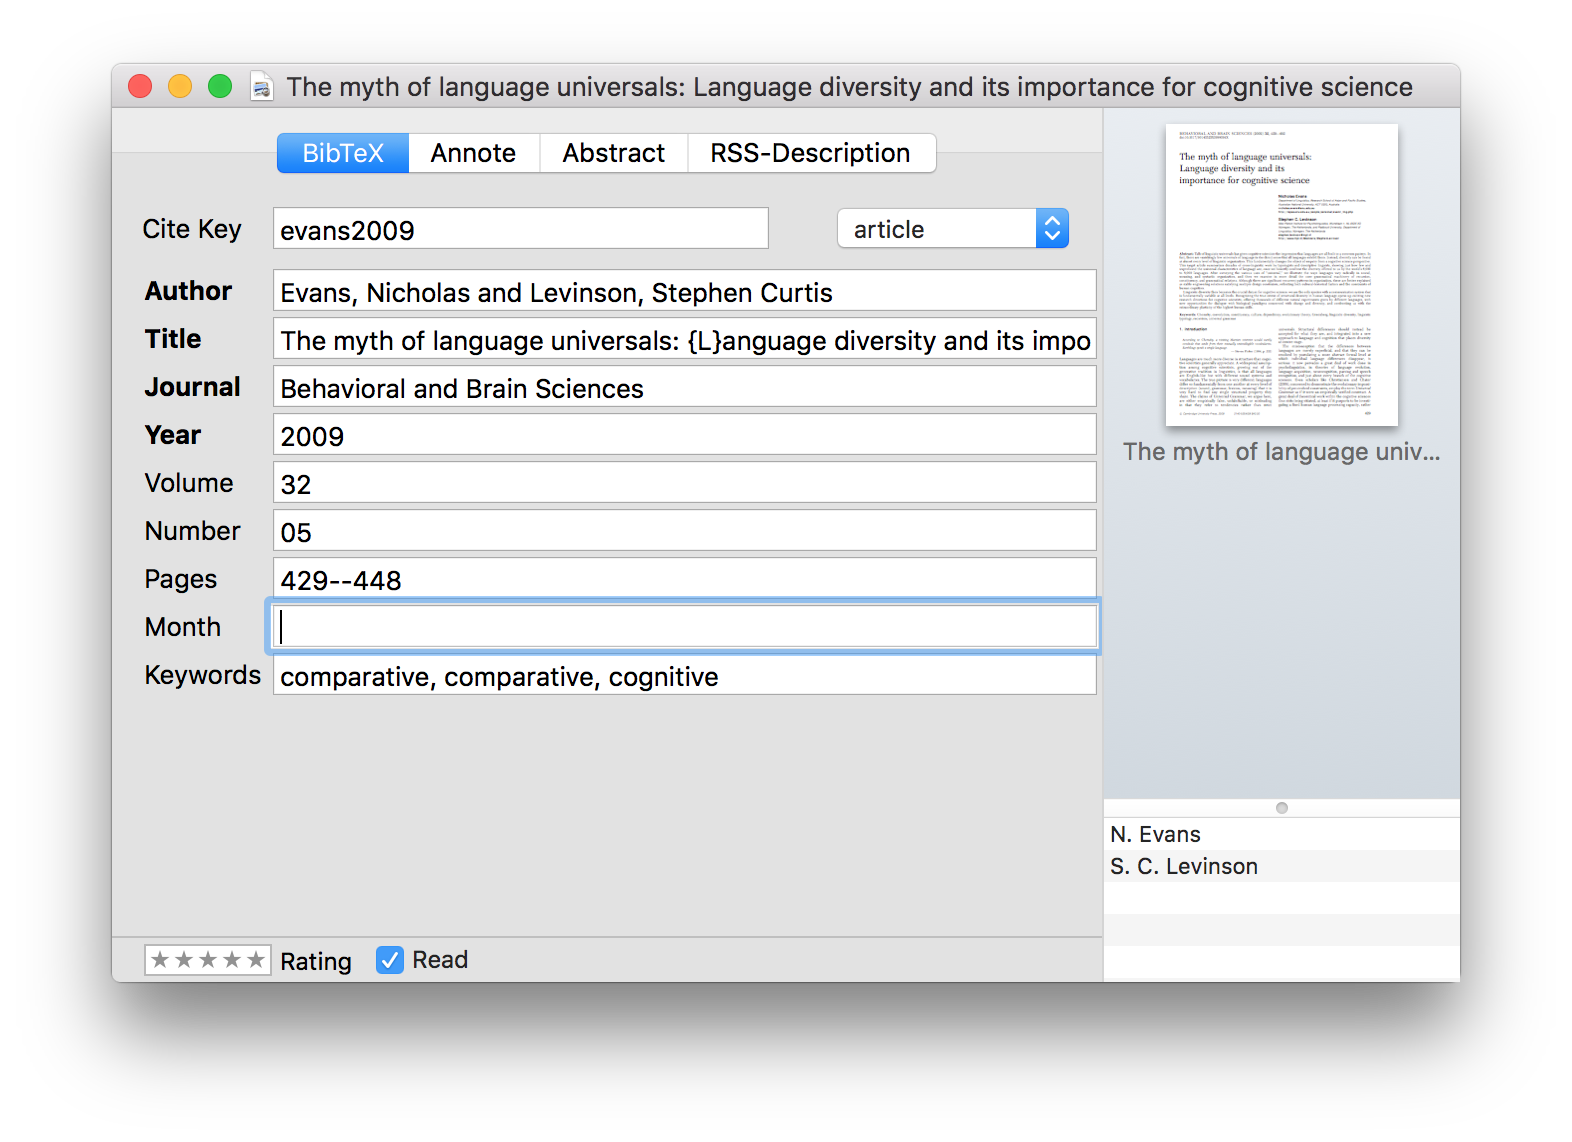
\includegraphics[width=0.9\textwidth]{entry}
\label{f:bibdesk}
\end{figure}

\end{frame}

%%%%%%%%%%%%%%%%%%%%%%%%%%%%%%%%%%%


\begin{frame}[fragile]
    \frametitle{The \texttt{natbib} package}

Load the \texttt{natbib} package in the preamble, with the option \texttt{numbers} for IEEE like style:
\begin{lstlisting}
\usepackage[numbers]{natbib}
\end{lstlisting}

Set the bibliography style (\texttt{plainnat}) and \texttt{.bib} file at the end of your document, before \verb+\end{document}+

\begin{lstlisting}
\bibliographystyle{plainnat}
\bibliography{mybib}
\end{lstlisting}

\end{frame}

%%%%%%%%%%%%%%%%%%%%%%%%%%%%%%%%%%%

\begin{frame}[fragile]
	\frametitle{The \texttt{natbib} package}
	
Call the \texttt{natbib} package in the preamble, with the option \texttt{numbers} for Harvard like style:
\begin{lstlisting}
\usepackage{natbib}
\end{lstlisting}

Set the bibliography style (\texttt{dcu}) and \texttt{.bib} file at the end of your document, before \verb+\end{document}+

\begin{lstlisting}
\bibliographystyle{dcu}
\bibliography{mybib}
\end{lstlisting}


\end{frame}

%%%%%%%%%%%%%%%%%%%%%%%%%%%%%%%%%%%

\begin{frame}
    \frametitle{The \texttt{natbib} package}

According to \textbf{Darwin (1859)}, we have a common ancestor with [...]. However, it is more complex \textbf{(Asimov 1951)}. As \textbf{Darwin (1859, p. 33--37}) said: ``This is the ultimate proof that [..].''

\end{frame}

%%%%%%%%%%%%%%%%%%%%%%%%%%%%%%%%%%%

\begin{frame}[fragile]
    \frametitle{The \texttt{natbib} package}

In your document, you can use the \verb+\cite+ commands:

\begin{lstlisting}
According to \citet{darwin1859}, we have a common ancestor with [...]. However, it is more complex \citep{asimov1951}.

As \citet[p. 33--37]{darwin1859} said: ``This is the ultimate proof that [..].''
\end{lstlisting}

The output depends on the chosen style. A Reference section will be automatically added at the end of your compiled document (PDF).

\end{frame}

%%%%%%%%%%%%%%%%%%%%%%%%%%%%%%%%%%%

\begin{frame}
    \frametitle{Style: \texttt{numeric}}

\begin{figure}
    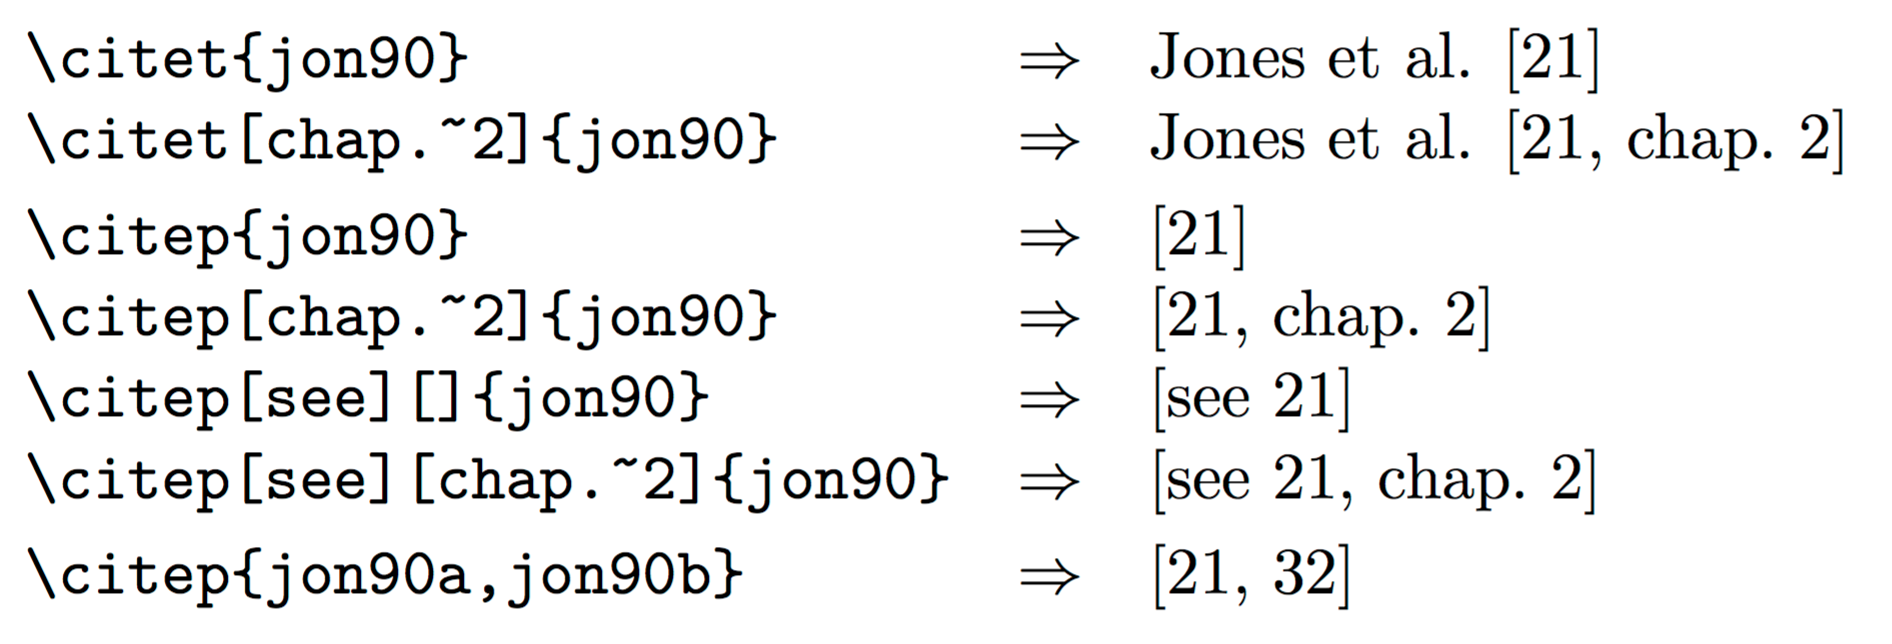
\includegraphics[width=\textwidth]{natbib-num}
\end{figure}


\end{frame}

%%%%%%%%%%%%%%%%%%%%%%%%%%%%%%%%%%%

\begin{frame}
    \frametitle{Style: \texttt{author-year}}

\begin{figure}
    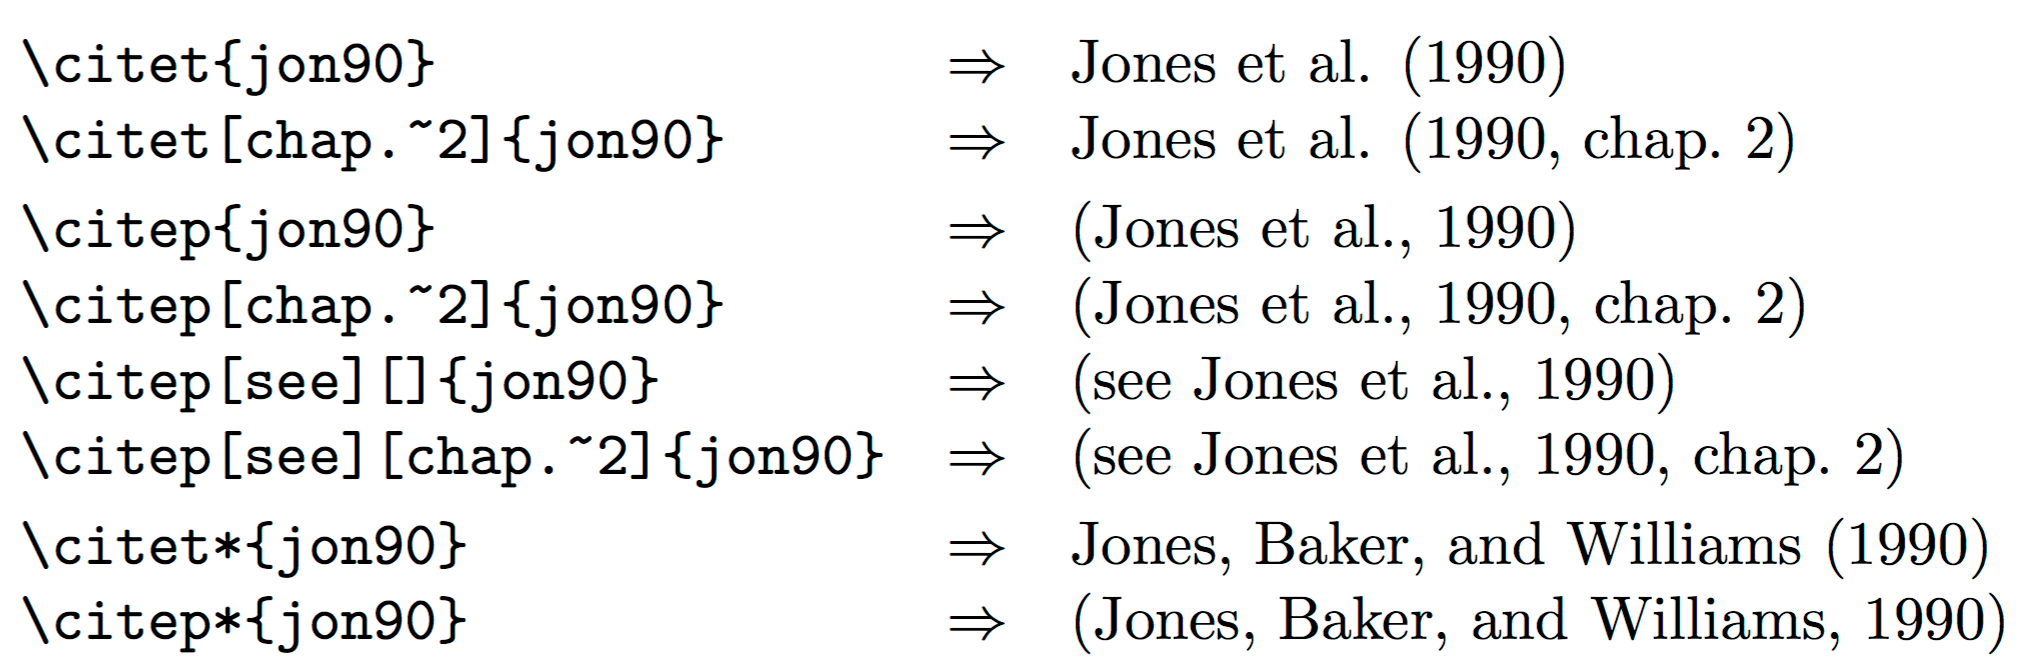
\includegraphics[width=\textwidth]{natbib-ay}
\end{figure}


\end{frame}

%%%%%%%%%%%%%%%%%%%%%%%%%%%%%%%%%%%













\end{document}
